\newpage
\section{Первоначальная настройка GNS3}

Установить GNS3 можно с официального сайта - \url{http://www.gns3.com/}. Для deb-like систем (Debian, Ubuntu, Mint) GNS3 доступен прямо из репозитория.

\begin{Verbatim}[frame=single]
apt-get install gns3
\end{Verbatim}

Первый запуск программы сопровождается появлением окна c мастером установки (рис. 1), состоящим из трёх шагов:
\begin{enumerate}
  \item указание путей к образом ОС;
  \item проверка корректности путей из шага 1;
  \item добавление образов IOS.
\end{enumerate}

\begin{figure}[h!]
\centering
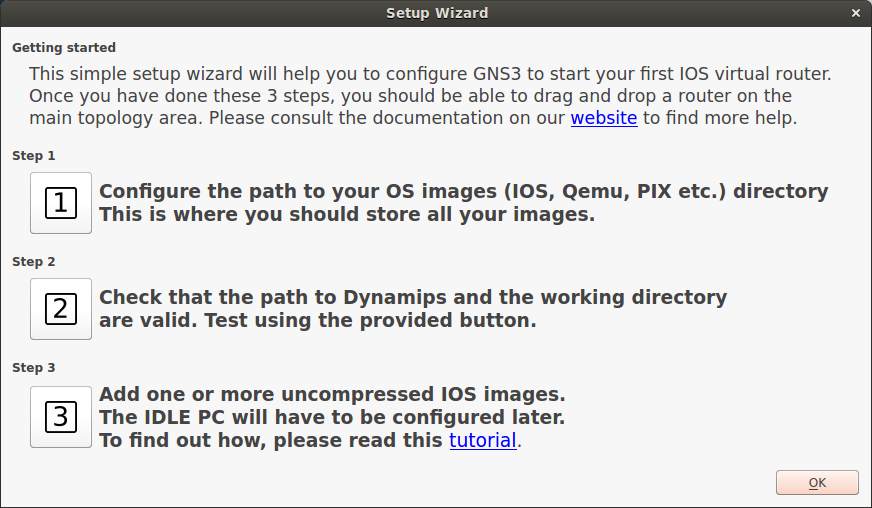
\includegraphics[scale=0.55]{res/pic001}
\caption{Мастер установки}
\end{figure}

От услуг этого мастера можно отказаться просто нажав "ОК" в правом нижнем углу.

Теперь перейдём к добавлению образов IOS. Их можно легко найти в интернете, на момент написания работы богатый выбор представлен на сайте \url{http://certs4u.info/ciscoios/c2650/c2691/}. Диалог добавления образа находится в меню Edit, пункт IOS images and hypervisors. Мы используем файл c2691-adventerprisek9\_sna-mz.124-13b.bin (это сжатый формат из которого можно получить c2691-adventerprisek9\_sna-mz.124-13b.image), а система автоматически определяет модель маршрутизатора (рис. 2).

\begin{figure}[h!]
\centering
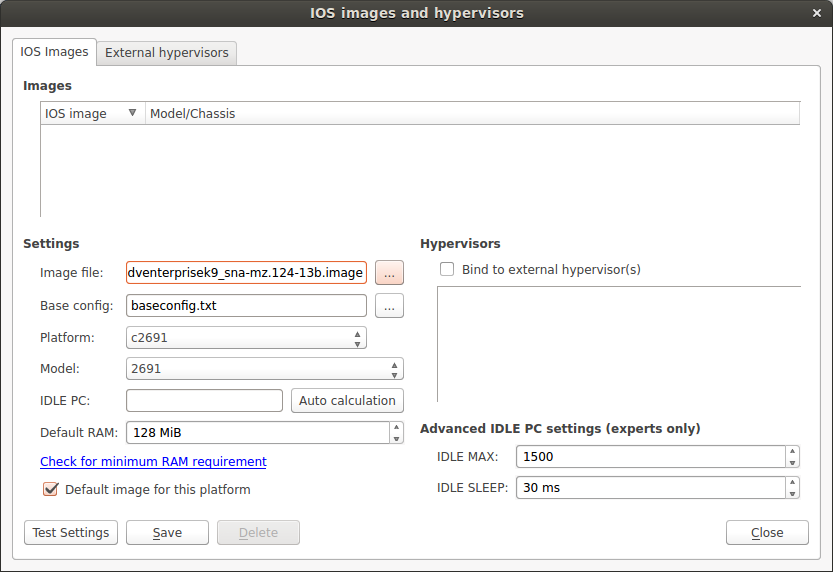
\includegraphics[scale=0.55]{res/pic002}
\caption{Диалог добавления образа IOS}
\end{figure}

Поле IDLE PC мы пока оставляем без внимания, вернёмся к нему позже.

Завершим работу диалога кнопкой Save и перейдём к диалогу создания нового проекта. Для его вызова, в меню File нужно выбрать пункт New blank project. В этом диалоге (рис. 3) важно выбрать пункт "Save nvrams including EtherSwitch VLANs and crypto keys".

\begin{figure}[h!]
\centering
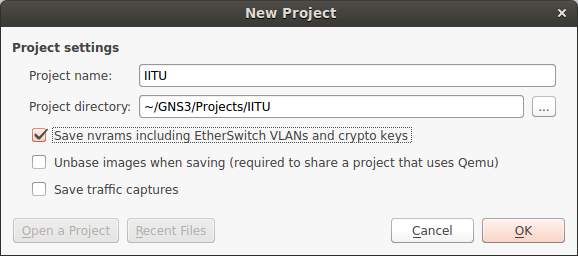
\includegraphics[scale=0.8]{res/pic003}
\caption{Диалог создания нового проекта}
\end{figure}

Этот пункт отвечает за сохранение конфигурации между перезапусками приложения.

Теперь добавим маршрутизатор на рабочую площадку (рис. 4) и запускаем его работу (пока с пустой конфигурацией).

\begin{figure}[h!]
\centering
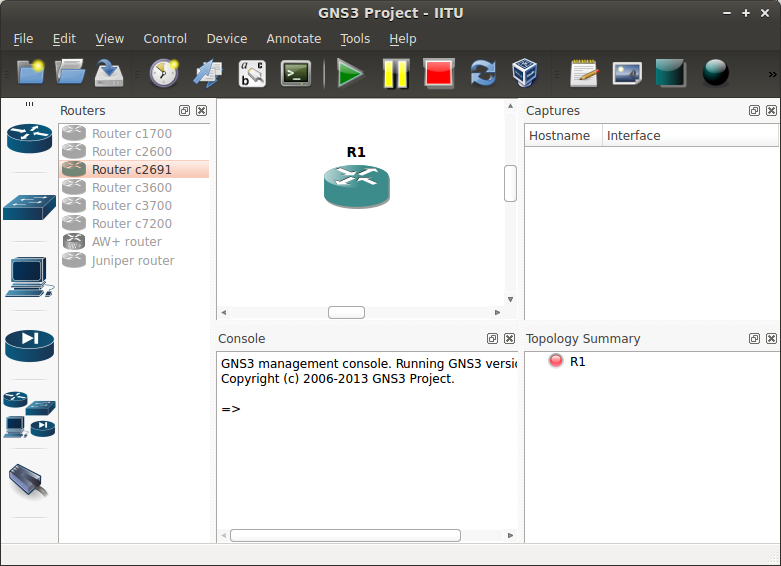
\includegraphics[scale=0.63]{res/pic004}
\caption{Диалог создания нового проекта}
\end{figure}

Это привело к колоссальной нагрузке на процессор -- 100\%!

\begin{Verbatim}[frame=single]
user@host:~$ top -b -n 1|grep dynamips
13909 user       20   0  553108 268408 197772 S 101,3  3,3   2:28.98 dynamips
\end{Verbatim}

Для оптимизации использования ресурсов процессов центрального процессора используется механизм IDLE PC, который мы ранее пропустили.

Его можно вызвать в контекстном меню, после чего система вычисляет несколько значений и предложит выбрать результат из списка. Рекомендуется выбирать значения со знаком * (рисунок 5). Как только они применяются, загрузка CPU падает (6,4\%).

\begin{Verbatim}[frame=single]
user@host:~$ top -b -n 1|grep dynamips
13909 user       20   0  553108 268408 197772 S   6,4  3,3  10:51.79 dynamips
\end{Verbatim}

\begin{figure}[h!]
\centering
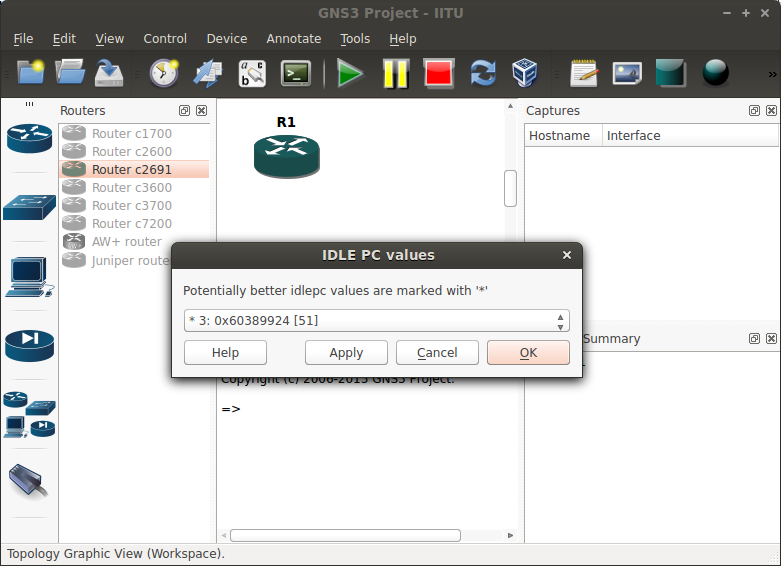
\includegraphics[scale=0.6]{res/pic005}
\caption{Оптимизация использования ресурсов CPU}
\end{figure}

Теперь можно подключиться к работающему роутеру. Для этого в контекстном меню нужно вызвать пункт console либо подключиться любим терминальным приложением к порту виртуального роутера через телнет. Номер порта можно узнать если навести мышку на роутер и немного подождать (рис. 6), либо через пункт Change console port контекстного меню.

\begin{figure}[h!]
\centering
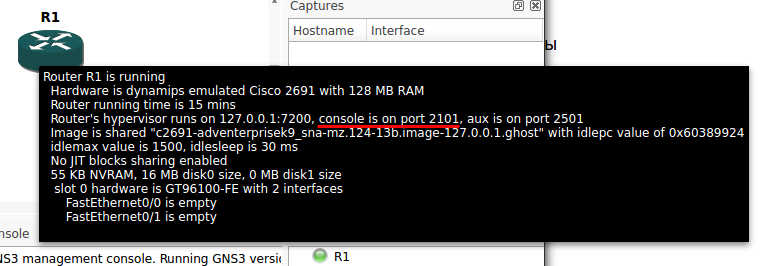
\includegraphics[scale=0.6]{res/pic006}
\caption{Определение номера порта консоли}
\end{figure}

Для подключения, нужно набрать команду
\begin{Verbatim}[frame=single]
telnet 127.0.0.1 2101
\end{Verbatim}

После чего появится доступ к управлению роутером (рис. 7).

\begin{figure}[h!]
\centering
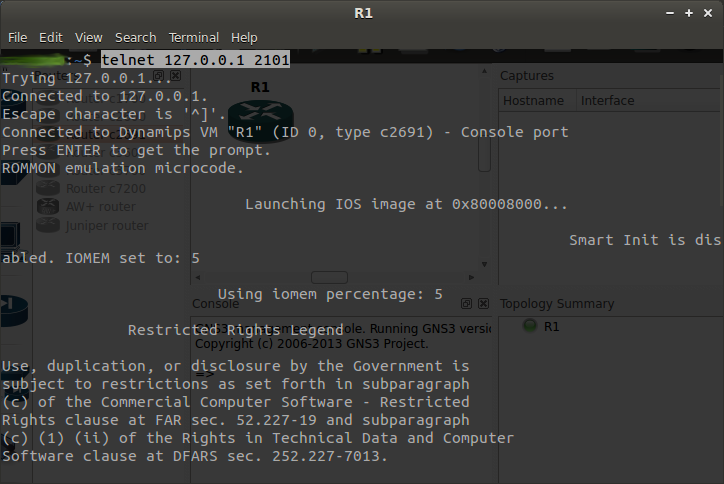
\includegraphics[scale=0.65]{res/pic007}
\caption{telnet подключение}
\end{figure}